\documentclass[tikz]{standalone}
\usepackage{pgfplots}
\pgfplotsset{compat=1.15}
\usepackage{mathrsfs}
\usetikzlibrary{arrows,calc}
\usepackage{tkz-euclide}
\pagestyle{empty}

\definecolor{AngleClr}{rgb}{0,0.39215686274509803,0}
\definecolor{ShapeClr}{rgb}{0.6,0.2,0}
\definecolor{BlueClr}{RGB}{52, 139, 207}

\begin{document}

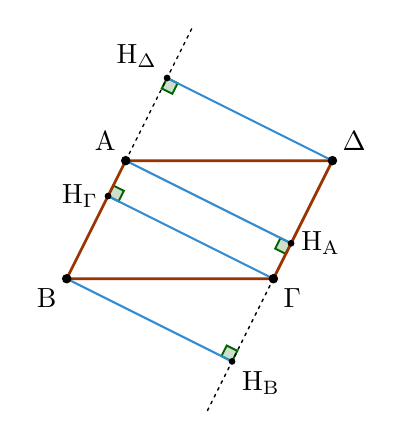
\begin{tikzpicture}[scale=.75]
\tkzSetUpLine[line width=1pt,color=black]
\tkzSetUpPoint[fill=black]

\tkzDefPoints{0/0/B,3.5/0/C,1/2/A,4.5/2/D}

\tkzInterLL(A,C)(B,D) \tkzGetPoint{O}
\tkzDefPointBy[projection = onto C--D](A) \tkzGetPoint{HA}
\tkzDefPointBy[projection = onto C--D](B) \tkzGetPoint{HB}
\tkzDefPointBy[projection = onto A--B](C) \tkzGetPoint{HC}
\tkzDefPointBy[projection = onto A--B](D) \tkzGetPoint{HD}

\tkzFillPolygon[fill=white](A,B,C,D)

\tkzMarkRightAngle[line width=0.7pt, size=.2,color=AngleClr,fill=AngleClr,fill opacity=0.2](A,HA,C)
\tkzMarkRightAngle[line width=0.7pt, size=.2,color=AngleClr,fill=AngleClr,fill opacity=0.2](B,HB,D)
\tkzMarkRightAngle[line width=0.7pt, size=.2,color=AngleClr,fill=AngleClr,fill opacity=0.2](C,HC,A)
\tkzMarkRightAngle[line width=0.7pt, size=.2,color=AngleClr,fill=AngleClr,fill opacity=0.2](D,HD,B)



\tkzDrawPolygon[color=ShapeClr](A,B,C,D)

\tkzDrawSegments[line width=0.75pt,color=BlueClr](A,HA B,HB C,HC D,HD)

\tkzDrawSegments[line width=0.5pt,color=black,dashed,dash pattern=on 1pt off 1.75pt,add=0 and 0.6](A,HD C,HB)


\tkzDrawPoints[size=3](A,B,C,D)
\tkzDrawPoints[size=2](HA,HB,HC,HD)

\tkzLabelPoint[above left](A){$\rm A$}
\tkzLabelPoint[below left](B){$\rm B$}
\tkzLabelPoint[below right](C){$\rm\Gamma$}
\tkzLabelPoint[above right](D){$\rm\Delta$}
\tkzLabelPoint[right](HA){$\rm H_A$}
\tkzLabelPoint[below right](HB){$\rm H_B$}
\tkzLabelPoint[left](HC){$\rm H_\Gamma$}
\tkzLabelPoint[above left](HD){$\rm H_\Delta$}

\end{tikzpicture}

\end{document}
